\chapter{\label{AN}Analysis Strategy}
% \begin{itemize}
%     \item Address all the basic questions.
%     \item write about all the simulations.
%     \item Add table on hoe you have applied cut
% \end{itemize}




The analysis done for the events where vector-like quark, $T’$, is produced after $PP$ collision at the CMS, LHC and further decays into a top quark and a Higgs boson, further decaying into two photons. We will be looking into the leptonic channel only. Further, we wish to set upper limits on the cross-section of the vector-like quark $T’$ with $M_{T’}$ in the range of [600, 1200] GeV.

The Higgs invariant mass (or di-photon invariant mass, $m_{\gamma\gamma}$ ) is the main probe of the analysis. The photons and di-photon Higgs candidates are reconstructed using the flashgg framework\cite{CrossSection_6}.
 Two mass regions are defined accordingly:
\begin{itemize}
    \item Signal window:  $m_{\gamma\gamma}$ $\in$ [115, 135]GeV
    \item Sideband region: $m_{\gamma\gamma}$ $\in$ [100, 115]$\cup$[135, 180]GeV
\end{itemize}
where the signal window is blinded throughout the development of the analysis.



Misclassification is less likely when optimal discrimination is used. In this regard, the typical method of selecting and applying cuts to one event variable at a time is rarely optimal. If correlations exist between a collection of event variables (denoted by a vector x), optimal separation may always be achieved if the variables are treated in a fully multivariate fashion. The best technique to partition a multidimensional space occupied by two classes of events, such as's' and 'b,' is to use a cut on the probability ratio,

\begin{equation}
    r(\textbf{x}) = \frac{p(s|\textbf{x})}{p(b|\textbf{x})} = \frac{p(\textbf{x}|s) p(s) }{p(\textbf{x}|b) p(b) }
\end{equation}

where  p(\textbf{x}|s) and p(\textbf{x}|b) are the class conditional probabilities, i.e., probability density functions for signal and background, and p(s) and p(b) are the prior probabilities.
 As a result, the posterior probability for the desired class's' is
 
\begin{equation}
    p(s|\textbf{x}) = \frac{r}{1+r} = \frac{ p(s|\textbf{x}) p(s)}{p(\textbf{x}|s)p(s) +  p(\textbf{x}|b)p(b)}
\end{equation}

The Bayes discriminant is the discriminant 'r'. Calculating the Bayes discriminant r(x) or the class conditional probabilities lowers the discrimination problem quantitatively. It's worth noting that, curiously, techniques like neural networks may directly produce the posterior probability p(s|\textbf{x}).



Here preselections are defined to maintain high efficiency in the signal events. To targets the leptonic decays of the top quark. These were done:-
\begin{enumerate}
    \item The binary classification algorithms (Deep Neural Network, DNN) with simulated samples of VLQ as signal and simulation of the related Standard Model processes as background with the following specifications, with one DNN is trained: only the Standard Model Higgs production modes are included as background during training.

\item Define a signal region by rectangular cuts on DNN scores. The cuts are determined such that the significance is maximized.

\item Construct parametric signal and background models from the fits to $m_{\gamma\gamma}$ distribution in each defined signal region. 
\item Non-resonant background are modeled from data in $m_{\gamma\gamma}$  sideband with a variety of functional from. The choice of functional from is treated as a discrete nuisance parameter, following the discrete profiling method. In particular, the fit is performed per mass point and per channel to capture the mass-dependent $m_{\gamma\gamma}$ resolution. In the end, we perform a simultaneous fit of the $m_{\gamma\gamma}$  spectra in the signal regions only for the leptonic channel to extract a limit on the cross-section for each mass point.
\end{enumerate}


When developing the analysis strategy for training classification algorithms, the idea of defining three $M_{T’}$ mass categories is proposed with the following practical considerations:
\begin{itemize}
    \item Kinematics of signal processes will be similar if $M_{T’}$ masses are not far different.
    \item Training 100 sets of DNNs would greatly increase the complexity of the analysis and also would increase training time and memory requirement.
\end{itemize}

Therefore, three mass ranges are defined such that signal samples are properly grouped for training:
\begin{itemize}
    \item $M_{T'} \in $[600, 700] GeV
    \item $M_{T'} \in $[800, 1000] GeV
    \item $M_{T'}   \in$ [1100, 1200]GeV
\end{itemize}


The input features of the training include the kinematic variables of all the final state particles. Since the kinematic features largely depend on $T'$mass, using one training for the whole mass range has been found sub-optimal in order to check a potential low $T'$ mass. Therefore three training is performed for different sets of $T'$ mass points [600, 625, 650, 675, 700], [800, 900, 1000], [1100, 1200]. The following are the list of variables used as the input features in the
training:
\begin{itemize}
    \item leading (sub-leading) photon pT/$m_{\gamma\gamma}$
    \item leading (sub-leading) photon photon IDMVA
    \item leading (sub-leading) pixel seed veto
    \item leading lepton charge, pT, $\eta$.
    \item Jet, b-jet and central jet( |$\eta$| < 1) multiplicity
    \item pT and |$\eta$| for leading two jets
    \item pT and b-tag score of the forward jet. The forward jet is the highest |$\eta$| jet in the event.
    \item angular separation between: each photon and the forward jet, the leading lepton,
\item leading b-jet and the forward jet
\end{itemize}


In each mass category, we follow the same analysis procedure presented above to derive final results. Beyond that, it is verified that searches for $T'$  mass situating between the mass categories (i.e. [700, 800] GeV and [1000, 1100] GeV) are also well described with this strategy. For each mass categories different DNN model have been trained.






% The $p\Bar{p}$ collision at the LHC, CERN provides events of interest altogether with another huge number of background processes. With the simulated sample of signals and backgrounds, which used for the training of the machine learning. The separation of signal and background is very tedious task in the experimental high energy physics. As can be seen in the fig. \autoref{fig:Signal_bkg_plotti}, both of the low level separation and high level separation features can not be separated with the raw samples. For the separation of the signal and background, the state level of art machine learning techniques can be used to separate the signals and backgrounds. Here, in the separation of the signal and background, the deep neural network(DNN) have been used, which have been discussed in the next sections.\\





% \section{simulation}








\section{DNN Model}
Deep neural network (DNN) is used here for training the data and further testing for the separation of signal and backgrounds. Keras module\cite{ml_1807}, Sequential\cite{ml_2}\cite{ml_3} used to make the DNN model. The model of the DNN used for the training is summaries in the table \autoref{tab:my_label_00}. 
%%%%%%%%%%%%%%%%%%%%%%%%%%%%%%%%%%%%%%%%%%%%%%%%%%%%%%%%%%%%%%%%%%%%%%%%%%%%%%%%%%%%%%%%%%%%%%%%%%%%%%%%%%%%%%%

\subsection{Model Preparation}
All the training and testing have been done in the jupyter notebook\cite{Kluyver2016jupyter}, python3 in the interface of lxplus as a CERN grid computing user. For the Ntuple in root to convert into array, it has been processed with the help of \textit{root2numpy}\cite{ml_4}\cite{noel_dawe_2017_842249}. There the total of 42 input variables in each sample of the signal and the SMH background ( \autoref{tab:my_label_Variable}) were in-focused which were provided to the DNN model. With further help of \textit{pandas Dataframe} \cite{reback2020pandas} the array converted into dataframe. The signal and background were divided into a single array which further before feeding the data into the DNN model. The signal were given the input as like ones and the background were given as the input as like zero. Further with the help of \textit{train\_test\_split}\cite{scikit-learn}, the data has been splitted as 33\% of the total dataset for the testing and rest for the training and validations. The training and testing have been done with three different models that is with Tprime[600-700 GeV], Tprime[800-1000 GeV], and Tprime[1100-1200 GeV], which have been discussed above. To prevent the training from over fitting the early stopping has been used by monitoring validation loss with the patience of 5 times of training. The overfitting decreases the accuracy of the model. There are different training techniques implemented according to the number of data points available\footnote{All the code related to this work can be found here: \url{https://github.com/raj2022/M.Sc.-thesis/tree/main/Codes}}. A generalized model for all the differnet training can be seen in the \autoref{tab:my_label_00}. As we are only doing binary classification as signal and background, we are using \textit{"RELU"} as the activation function between the input layer \& hidden layer, and hidden layer \& hidden layer. The activation function \textit{"Sigmoid"} have been used as output layer for the binary classification. To update the weights between the layer, the binary cross entopy loss function have been used, with \textit{"ADAM"} as the optimizer and giving matrices as the accuracy. The total training data(68\% of the total signal and background) were divide into batches of 9000, which run through the model for 100 times. 

\begin{table}[h!]
     \centering
     \resizebox{\textwidth}{!}{
     \begin{tabular}{|ccc|}\hline
       Options   &   & Description \\\hline
    Model      &    Sequential  &   -   \\
    Number of Inputs      &    42  &    as given in \autoref{tab:my_label_Variable}  \\
    Number of layers (Input)     & 512     &  $Dense\_1$    \\
        Hidden  &  512    &  $Dense\_2$    \\
         Hidden &  256    &   $Dense\_3$   \\
        Hidden  & 128     &  $Dense\_4$    \\
        Hidden  & 64     & $Dense\_5$     \\
           Hidden  & 32     & $Dense\_6$     \\
        Output  & 1      &  $Dense\_7$    \\
    Activation function(Hidden Layer)      &  ReLU    &   Same for both binary\\  
    & & classification and multiclassification   \\
      Activation layer(Output)    & sigmoid     &  For binary classification    \\
                                  &  Softmax  & For multi classification    \\
    Loss function   &   Binary cross entropy    & For binary classification \\
                    &    categorical\_crossentropy  & For multi classification \\
    Optimizer      &     ADAM     &     -\\
    Matrices     & Accuracy    &  \\
    BatchSize      & 9000  & Batch size used for a single gradient  \\
                      &    &     step during training  \\
    NumEpochs      & 100 &   Number of training epochs \\
    Verbose &    1  &  Verbosity during training \\\hline
    
     \end{tabular}}
     \caption{Configurations of the Keras model used for training and testing purposes}
     \label{tab:my_label_00}
 \end{table}
\hspace{3em}


\subsubsection{Tprime($T'$(600-700))}
For the training of this model there were total of 801,385 parameters out of which 796,629 was trainable parameters and 4,756 non-trainable parameters due to dropouts and normalization applied to each layer. The trained score were saved in the form of .h5 file and it was further used for testing on signals, standard model Higgs(SMH) background, and the non-resonant backgrounds(NRB). The testing and training adopted is summarised in \autoref{tab:model600-700}
\begin{table}[H]
    \centering
    \setlength{\tabcolsep}{16pt}
    \resizebox{\textwidth}{!}{
    \begin{tabular}{|c|c|c|}\hline
     MC type    &  Training Samples &    Testing Samples\\ \hline
      Signal      &  TprimeBToTH\_Hgg\_M-600\_LH\_TuneCP5\_PSweights\_13TeV-madgraph\_pythia8.root  &  TprimeBToTH\_Hgg\_M-600\_LH\_TuneCP5\_PSweights\_13TeV-madgraph\_pythia8.root \\ 
         &               &                 \\
               & TprimeBToTH\_Hgg\_M-625\_LH\_TuneCP5\_PSweights\_13TeV-madgraph\_pythia8.root & TprimeBToTH\_Hgg\_M-625\_LH\_TuneCP5\_PSweights\_13TeV-madgraph\_pythia8.root    \\
                        &               &                 \\

               & TprimeBToTH\_Hgg\_M-650\_LH\_TuneCP5\_PSweights\_13TeV-madgraph\_pythia8.root & TprimeBToTH\_Hgg\_M-650\_LH\_TuneCP5\_PSweights\_13TeV-madgraph\_pythia8.root    \\
                        &               &                 \\

               & TprimeBToTH\_Hgg\_M-675\_LH\_TuneCP5\_PSweights\_13TeV-madgraph\_pythia8.root &  
               TprimeBToTH\_Hgg\_M-650\_LH\_TuneCP5\_PSweights\_13TeV-madgraph\_pythia8.root\\
                        &               &                 \\

               & TprimeBToTH\_Hgg\_M-700\_LH\_TuneCP5\_PSweights\_13TeV-madgraph\_pythia8.root &   
               TprimeBToTH\_Hgg\_M-700\_LH\_TuneCP5\_PSweights\_13TeV-madgraph\_pythia8.root\\
                        &               &                 \\
\hline \hline
    
    
    SMH    &      ttHJetToGG\_M125\_13TeV\_amcatnloFXFX\_madspin\_pythia8.root  &       \\   
             &               &                 \\

          &      THQ\_ctcvcp\_HToGG\_M125\_13TeV-madgraph-pythia8.root  &       \\ 
                   &               &                 \\


          &     GluGluHToGG\_M125\_TuneCP5\_13TeV-amcatnloFXFX-pythia8.root  &   All Combined     \\ 
                   &               &                 \\


          &      VBFHToGG\_M125\_13TeV\_amcatnlo\_pythia8.root  &       \\ 
                   &               &                 \\


          &      VHToGG\_M125\_13TeV\_amcatnloFXFX\_madspin\_pythia8.root &       \\
                   &               &                 \\

\hline \hline
  
  
 NRB   &     &    output\_TTJets\_pythia8.root            \\ 
          &               &                 \\

       &   &  output\_TTGG\_0Jets\_pythia8.root     \\
                &               &                 \\

       &  & output\_TGJets\_pythia8.root \\
                &               &                 \\

       &  & output\_GJet\_Pt-40toInf\_DoubleEMEnriched\_MGG-80toInf\_pythia8.root \\
                &               &                 \\

       &  & output\_DiPhotonJetsBox\_MGG-80toInf\_13TeV-Sherpa.root \\ \hline
    \end{tabular}}
    \caption{Training with Tprime[600-700GeV] and testing done on Tprime at 600 GeV, 700 GeV, SMH backgrounds, and NRB backgrounds.}
    \label{tab:model600-700}
\end{table}

\subsubsection{Tprime($T'$(800-1000))}

For the training of this model there were total of 749,609 parameters out of which 746,517 was trainable parameters and 3,092 non-trainable parameters due to dropouts and normalization applied to each layer. The trained score were saved in the form of .h5 file and it was further used for testing on signals, standard model Higgs(SMH) background, and the non-resonant backgrounds(NRB). The testing and training adopted can be summarised as similarly in \autoref{tab:model600-700}.


% \begin{table}[H]
%     \centering
%     \resizebox{\textwidth}{!}{
%     \begin{tabular}{|c|c|c|}\hline
%      MC type    &  Training Samples &    Testing Samples\\ \hline
%       Signal      &  TprimeBToTH\_Hgg\_M-700\_LH\_TuneCP5\_PSweights\_13TeV-madgraph\_pythia8.root  &  TprimeBToTH\_Hgg\_M-600\_LH\_TuneCP5\_PSweights\_13TeV-madgraph\_pythia8.root \\ 
%          &               &                 \\
%               & TprimeBToTH\_Hgg\_M-900\_LH\_TuneCP5\_PSweights\_13TeV-madgraph\_pythia8.root & TprimeBToTH\_Hgg\_M-700\_LH\_TuneCP5\_PSweights\_13TeV-madgraph\_pythia8.root    \\
%                         &               &                 \\

%               & TprimeBToTH\_Hgg\_M-1000\_LH\_TuneCP5\_PSweights\_13TeV-madgraph\_pythia8.root & TprimeBToTH\_Hgg\_M-800\_LH\_TuneCP5\_PSweights\_13TeV-madgraph\_pythia8.root    \\
%                         &               &                 \\

%               &  &  
%               TprimeBToTH\_Hgg\_M-900\_LH\_TuneCP5\_PSweights\_13TeV-madgraph\_pythia8.root\\
%                         &               &                 \\

%               &  &   
%               TprimeBToTH\_Hgg\_M-1000\_LH\_TuneCP5\_PSweights\_13TeV-madgraph\_pythia8.root\\
%                         &               &                 \\
% \hline \hline
    
    
%     SMH    &      ttHJetToGG\_M125\_13TeV\_amcatnloFXFX\_madspin\_pythia8.root  &       \\   
%              &               &                 \\

%           &      THQ\_ctcvcp\_HToGG\_M125\_13TeV-madgraph-pythia8.root  &       \\ 
%                   &               &                 \\


%           &     GluGluHToGG\_M125\_TuneCP5\_13TeV-amcatnloFXFX-pythia8.root  &   All Combined     \\ 
%                   &               &                 \\


%           &      VBFHToGG\_M125\_13TeV\_amcatnlo\_pythia8.root  &       \\ 
%                   &               &                 \\


%           &      VHToGG\_M125\_13TeV\_amcatnloFXFX\_madspin\_pythia8.root &       \\
%                   &               &                 \\

% \hline \hline
  
  
%  NRB   &    &    output\_TTJets\_pythia8.root            \\ 
%           &               &                 \\

%       &     &  output\_TTGG\_0Jets\_pythia8.root     \\
%                 &               &                 \\

%       & & output\_TGJets\_pythia8.root \\
%                 &               &                 \\

%       &  & output\_GJet\_Pt-40toInf\_DoubleEMEnriched\_MGG-80toInf\_pythia8.root \\
%                 &               &                 \\

%       & & output\_DiPhotonJetsBox\_MGG-80toInf\_13TeV-Sherpa.root \\ \hline
%     \end{tabular}}
%     \caption{Training with Tprime[800-1000GeV] and testing done on Tprime at 600GeV, 700GeV, 800 GeV,
% 900 GeV, 1000GeV SMH backgrounds, and NRB backgrounds.}
%     \label{tab:model800-1100}
% \end{table}


\subsubsection{Tprime($T'$(1100-1200))}
For the training of this model there were total of  266,537 parameters out of which 264,469 was trainable parameters and 2,068 non-trainable parameters due to dropouts and normalization applied to each layer. The trained score were saved in the form of .h5 file and it was further used for testing on signals, standard model Higgs(SMH) background, and the non-resonant backgrounds(NRB). The testing and training adopted can be summarised as similarly in \autoref{tab:model600-700}.

% \begin{table}[H]
%     \centering
%     \resizebox{\textwidth}{!}{
%     \begin{tabular}{|c|c|c|}\hline
%      MC type    &  Training Samples &    Testing Samples\\ \hline
%       Signal      &  TprimeBToTH\_Hgg\_M-1100\_LH\_TuneCP5\_PSweights\_13TeV-madgraph\_pythia8.root  &  TprimeBToTH\_Hgg\_M-600\_LH\_TuneCP5\_PSweights\_13TeV-madgraph\_pythia8.root \\ 
%          &               &                 \\
%               & TprimeBToTH\_Hgg\_M-1200\_LH\_TuneCP5\_PSweights\_13TeV-madgraph\_pythia8.root & TprimeBToTH\_Hgg\_M-700\_LH\_TuneCP5\_PSweights\_13TeV-madgraph\_pythia8.root    \\
%                         &               &                 \\

%               &  & TprimeBToTH\_Hgg\_M-900\_LH\_TuneCP5\_PSweights\_13TeV-madgraph\_pythia8.root    \\
%                         &               &                 \\

%               &  &  
%               TprimeBToTH\_Hgg\_M-1100\_LH\_TuneCP5\_PSweights\_13TeV-madgraph\_pythia8.root\\
%                         &               &                 \\

%               &  &   
%               TprimeBToTH\_Hgg\_M-1200\_LH\_TuneCP5\_PSweights\_13TeV-madgraph\_pythia8.root\\
%                         &               &                 \\
                        
                        
% \hline \hline
    
    
%     SMH    &      ttHJetToGG\_M125\_13TeV\_amcatnloFXFX\_madspin\_pythia8.root  &       \\   
%              &               &                 \\

%           &      THQ\_ctcvcp\_HToGG\_M125\_13TeV-madgraph-pythia8.root  &       \\ 
%                   &               &                 \\


%           &     GluGluHToGG\_M125\_TuneCP5\_13TeV-amcatnloFXFX-pythia8.root  &   All Combined     \\ 
%                   &               &                 \\


%           &      VBFHToGG\_M125\_13TeV\_amcatnlo\_pythia8.root  &       \\ 
%                   &               &                 \\


%           &      VHToGG\_M125\_13TeV\_amcatnloFXFX\_madspin\_pythia8.root &       \\
%                   &               &                 \\

% \hline \hline
  
  
%  NRB   &       &    output\_TTJets\_pythia8.root            \\ 
%           &               &                 \\

%       &     &  output\_TTGG\_0Jets\_pythia8.root     \\
%                 &               &                 \\

%       &  & output\_TGJets\_pythia8.root \\
%                 &               &                 \\

%       &   & output\_GJet\_Pt-40toInf\_DoubleEMEnriched\_MGG-80toInf\_pythia8.root \\
%                 &               &                 \\

%       & & output\_DiPhotonJetsBox\_MGG-80toInf\_13TeV-Sherpa.root \\ \hline
%     \end{tabular}}
%     \caption{Training with Tprime[1100-1200GeV] and testing done on Tprime at 600 GeV,
% 700 GeV, 1100 GeV, 1200 GeV, SMH backgrounds, and NRB backgrounds.}
%     \label{tab:model1100-1200}
% \end{table}

\section{Training Model Output}
The training output from different DNN model can be seen in the \autoref{fig:output_training_models}.


\begin{figure}[H]
     \centering
     \begin{subfigure}[b]{0.47\textwidth}
         \centering
         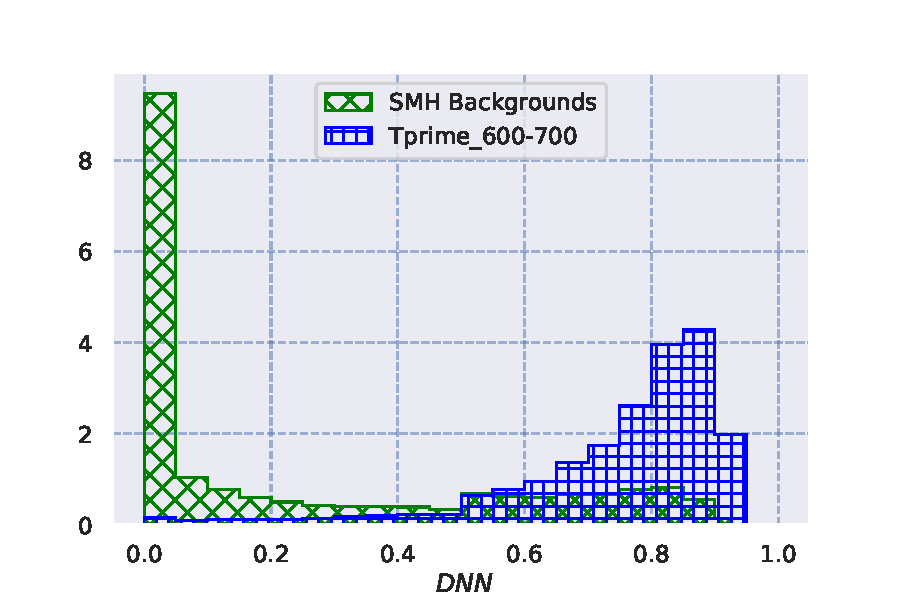
\includegraphics[width=\textwidth]{figure_4/output_TPrime600-700_on_testing_all_background.pdf}
         \caption{Tprime(600-700GeV)}
         \label{fig:y equals x}
     \end{subfigure}
     \hfill
     \begin{subfigure}[b]{0.47\textwidth}
         \centering
         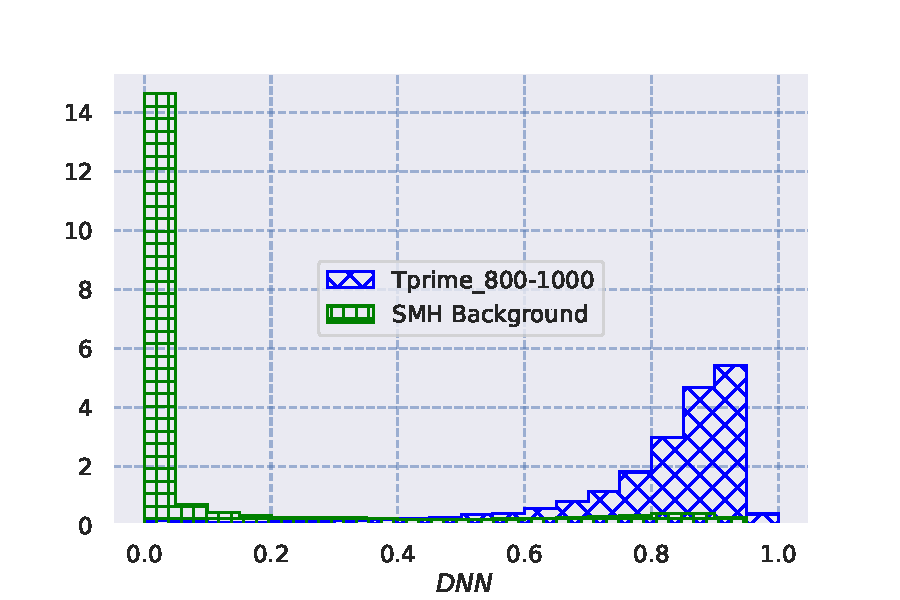
\includegraphics[width=\textwidth]{figure_4/output_TPrime800-1000_on_testing_all_background.pdf}
         \caption{Tprime(800-1000GeV)}
         \label{fig:three sin x}
     \end{subfigure}
     \hfill
     \begin{subfigure}[b]{0.47\textwidth}
         \centering
         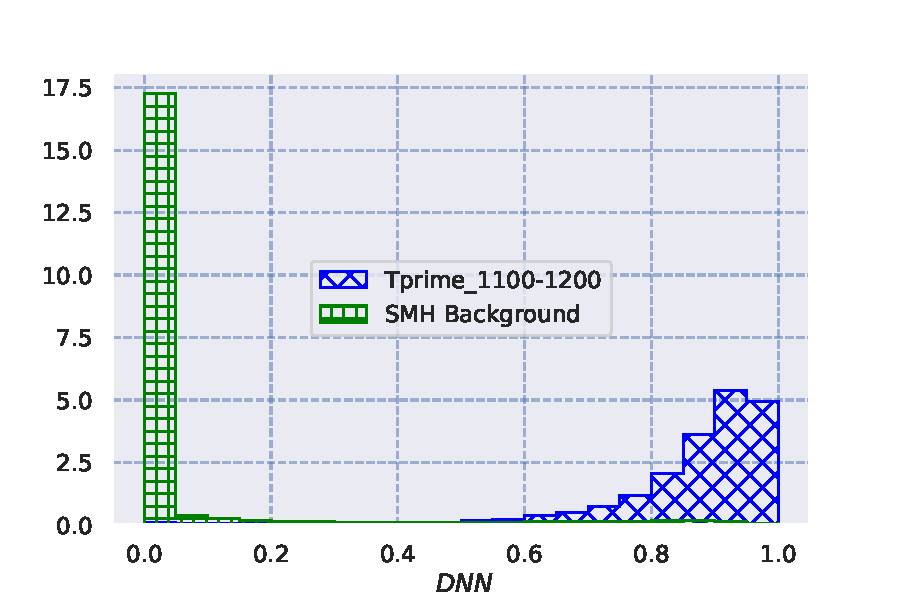
\includegraphics[width=\textwidth]{figure_4/Training_with_Tprime_1100-1200GeV_ with_backgrounds.pdf}
         \caption{Tprime(1100-1200GeV)}
         \label{fig:five over x}
     \end{subfigure}
        \caption{Separation output of signal $T{'}$ from the background after all different training in all three mass point of $T{'}$}
        \label{fig:output_training_models}
\end{figure}


To check the model training output, the corresponding output from the model has been plotted with the help of validation dataset accuracy and loss on the model. The loss of model can be interpreted as the following theoretical loss and accuracy plots as in \autoref{fig:training_and_accuracy_theo}.

\begin{figure}[H]
     \centering
     \begin{subfigure}[b]{0.4\textwidth}
         \centering
         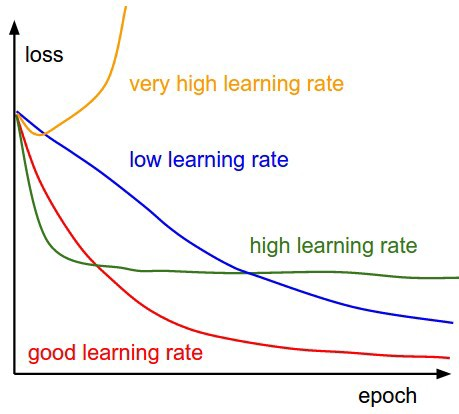
\includegraphics[width=\textwidth]{figure_4/loss.jpeg}
         \caption{loss from trained output model}
         \label{fig:y equals x}
     \end{subfigure}
     \hfill
     \begin{subfigure}[b]{0.4\textwidth}
         \centering
         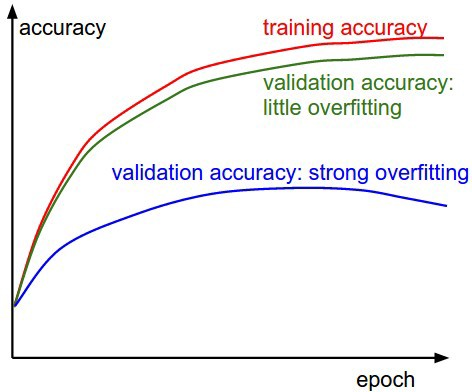
\includegraphics[width=\textwidth]{figure_4/accuracy.jpeg}
         \caption{Corresponding Accuracy}
         \label{fig:three sin x}
     \end{subfigure}

        \caption{Theoretical loss and accuracy plots\cite{ml_68}}
        \label{fig:training_and_accuracy_theo}
\end{figure}



From the \autoref{fig:output_training_models}, the model would giving a clear separation between signal and background for each model of training. Using the DNN output score, the diffent samples as discussed above were tested and output has been plotted in \autoref{fig:my_label_fig_testing}
\begin{figure}[H]
    \centering
    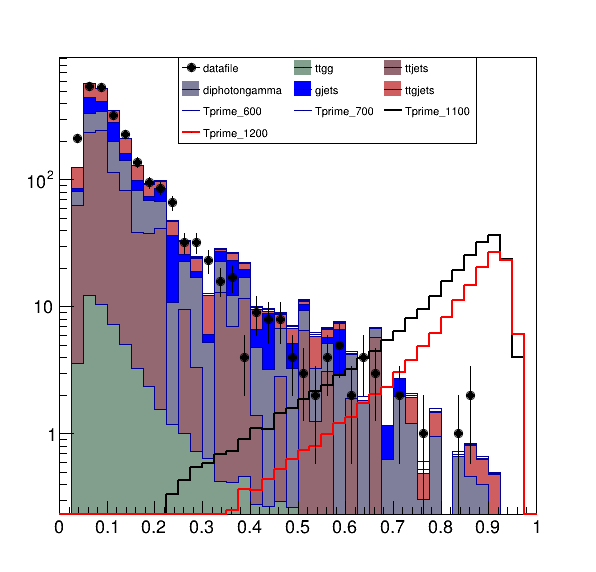
\includegraphics[scale=0.4]{Results_outputs/output_After_testing.png}
    \caption{Output after testing the model on the datafile, NRB, SMH, and Signals.}
    \label{fig:my_label_fig_testing}
\end{figure}



With applying weights to the input of the root file the stacked ratio plotted. To prevented the data and montecarlo mismatch, the histogram have been re-scaled with \textit{DataYield/ totalMCYield}.
 This confirms the data and monte carlo comparisons as in \autoref{fig:my_label_fig_testing}. If the data and monte carlo have mismatch then either there might be a few depressions in the data or we need to modify the theoretical predictions. 
 %%%%%%%%%%%%%%%%%%%%%%%%%%%%%%%%%%%%%%%%%%%%%%%%%%%%%%%%%$$$$$$$$$$$$$$$$$$$$$$$$$$$$$$$$$$$$$$$$$$$$$$$$$$$$$$$$$$$$$$$$$$$$$$$$$$%%%%%%%%%%%%%%%%%%%%%%%%%%%%%%%%%%%%%%%%%%%%%%%%%%%%%%%%%%%%%%%%%%%%%%%%%%%%%%%%%%%%%%%%%%%%%%%%%%%%%%%%%%%%%%%%%%%%%%%%%%%%%%%%%%%%%%%%%%%%%%%%%%%%%%%%%%%%%%%%%%%%%%%%%%%%%%
On the DNN output from each mass points of T$'$ from [600, 1200], expected limit have been calculated which has been discussed in details in \autoref{sec:limit_Ca}. 
As discussed above, a similar procedure have been adopted for another machine learning techniques(Boosted decision tree(BDT)) from ongoing analysis(adopted from a publicly available analysis in CMS, CERN) for comparison of the output and check for a better sensitivity. The output after testing on both the model have been plotted in \autoref{sec:comp}.



\setcounter{equation}{0}
\setcounter{table}{0}
\setcounter{figure}{0}
%\baselineskip 24pt


    
           


 




 
 
